\documentclass{beamer}
%\usepackage[margin=1.0in]{geometry}

\usepackage[utf8]{inputenc}
\usepackage[english]{babel}
\usepackage[T1]{fontenc}
\usepackage{lmodern}

%----------------------------------------------------------------------------------------
%	MATH PACKAGES
%----------------------------------------------------------------------------------------

% Banish \phi from this realm
\renewcommand{\phi}{\varphi}

\usepackage{amsmath, amssymb, mathrsfs}
\usepackage{mathtools}

%----------------------------------------------------------------------------------------
%	DEFINING NEW FUNCTIONS
%----------------------------------------------------------------------------------------

% --------- MATH MODE ---------
% Equation numbering per section
%\numberwithin{equation}{section}

% \cdot instead of asterisk (*) symbol
\mathcode`\*="8000
{\catcode`\*\active\gdef*{\cdot}}

% --------- OTHER ---------

% tikz
\usepackage{tikz}

% Captions
\usepackage[font=scriptsize]{caption}

% Quotes
\usepackage[autostyle=false]{csquotes}
\newcommand{\q}[1]{„#1''} % Redefine quotations

\usetheme{Madrid}
\usecolortheme{default}
\setbeamertemplate{caption}[numbered]

\newif\ifplacelogo
\placelogotrue
%----------------------------------------------------------------------------------------
%	TITLE PAGE
%----------------------------------------------------------------------------------------
\title[Limitations on rotation and radius of NS]
{Limitations on rotation and radius of NS}
\subtitle{A presentation based on Glendenning's Compact Stars}

\author[Balázs Pál]
{Balázs Pál}

\institute[ELTE]
{Eötvös Loránd University}

\date[ELTE 2022]
{The structure of compact stars\\June 13, 2022}

\logo{\ifplacelogo\tikz\node[opacity=0.3,inner sep=2pt] {
\includegraphics[height=1.1cm]{./images/elte-logo.png}};\fi}

\begin{document}

\frame{\titlepage}
%----------------------------------------------------------------------------------------
%	SLIDE 1.
%----------------------------------------------------------------------------------------
\begin{frame}
\frametitle{Overview}

\begin{itemize}
	\item The Kepler frequency is just an absolute limit: other limitaions may occur that sets an upper limit below $\Omega_{K}$.
\end{itemize}

\end{frame}
%----------------------------------------------------------------------------------------
%	SLIDE 2.
%----------------------------------------------------------------------------------------
\begin{frame}
\frametitle{Frame-dragging}
\framesubtitle{Effect of rotation on metric tensor}

\begin{itemize}
	\item The metric tensor in case of a static, stationary star is described in the Schwarzschield metric with $G = c = 1$ contains only diagonal elements
	\begin{block}{}
		\begin{equation} \label{eq:1}
		\begin{aligned}
			g
			=
			d \tau^{2}
			=
			e^{2 \nu \left( r \right)} dt^{2}
			-
			e^{2 \lambda \left( r \right)} dr^{2}
			-
			r^{2} d \theta^{2}
			-
			r^{2} sin^{2} \left( \theta \right) d \phi^{2}
		\end{aligned}
		\end{equation}
	\end{block}
	\item Rotation however introduces off-diagonal elements too (where $\omega \neq 0$ is the angular velocity of local interial frames)
	\begin{block}{}
		\begin{equation} \label{eq:2}
		\begin{aligned}
			g
			=
			d \tau^{2}
			=&
			\ e^{2 \nu \left( r, \theta \right)} dt^{2}
			-
			e^{2 \lambda \left( r, \theta \right)} dr^{2} 
			\\
			&-
			e^{2 \mu \left( r, \theta \right)}
			\left[
				r^{2} d \theta^{2} + r^{2} \sin^{2} \left( \theta \right)
				*
				\left(
					d \phi - \omega \left( r, \theta \right) dt
				\right)^{2}
			\right]
		\end{aligned}
		\end{equation}
	\end{block}
	\item Due to rotation the star deforms around the equator (centrifugal flattening) and loses spherical symmetry
\end{itemize}

\end{frame}
%----------------------------------------------------------------------------------------
%	SLIDE 2.
%----------------------------------------------------------------------------------------
\begin{frame}
\frametitle{Frame-dragging}
\framesubtitle{Effect of rotation on metric tensor}

\begin{itemize}
	\item The metric tensor in case of a static, stationary star is described in the Schwarzschield metric with $G = c = 1$ contains only diagonal elements
	\begin{block}{}
		\begin{equation} \label{eq:1}
		\begin{aligned}
			g
			=
			d \tau^{2}
			=
			e^{2 \nu \left( r \right)} dt^{2}
			-
			e^{2 \lambda \left( r \right)} dr^{2}
			-
			r^{2} d \theta^{2}
			-
			r^{2} sin^{2} \left( \theta \right) d \phi^{2}
		\end{aligned}
		\end{equation}
	\end{block}
	\item Rotation however introduces off-diagonal elements too (where $\omega \neq 0$ is the angular velocity of local interial frames)
	\begin{block}{}
		\begin{equation} \label{eq:2}
		\begin{aligned}
			g
			=
			d \tau^{2}
			=&
			\ e^{2 \nu \left( r, \theta \right)} dt^{2}
			-
			e^{2 \lambda \left( r, \theta \right)} dr^{2} 
			\\
			&-
			e^{2 \mu \left( r, \theta \right)}
			\left[
				r^{2} d \theta^{2} + r^{2} \sin^{2} \left( \theta \right)
				*
				\left(
					d \phi - \omega \left( r, \theta \right) dt
				\right)^{2}
			\right]
		\end{aligned}
		\end{equation}
	\end{block}
	\item Due to rotation the star deforms around the equator (centrifugal flattening) and loses spherical symmetry
\end{itemize}

\end{frame}
%----------------------------------------------------------------------------------------
%	SLIDE 3.
%----------------------------------------------------------------------------------------
\begin{frame}
\frametitle{Kepler frequency in GR}

\begin{itemize}
	\item To only unknown in Eq. \eqref{eq:2} is the $V$ velocity of a fluid element along the equator. This can be determined by finding the extremum of
	\begin{block}{}
		\begin{equation} \label{eq:3}
			\mathrm{d}\tau
			=
			\int_{t_{1}}^{t_{2}} \mathrm{d}t\,
			\sqrt{
				e^{2 \nu} - r^{2} e^{2 \mu} \left( \Omega - \omega \left( R \right) \right)^{2}
			}
		\end{equation}
	\end{block}
	\item After solving the variational problem and expanding $V$, we get the solution as
	\begin{block}{}
		\begin{equation} \label{eq:4}
			V_{\pm}
			=
			\frac{R \omega'}{2 \psi'} e^{\mu - \nu}
			\pm
			\sqrt{
				\frac{\nu'}{\psi'}
				+
				\left(
					\frac{R \omega'}{2 \psi'} e^{\mu - \nu}
				\right)^{2}
			},
		\end{equation}
	\end{block}
	where $\psi' = \mu' + 1 / R$
	\item The physically interesting result is given by $V_{+}$, since that is the co-rotating case needed for Eq. \eqref{eq:2}.
\end{itemize}

\end{frame}
%----------------------------------------------------------------------------------------
%	SLIDE 5.
%----------------------------------------------------------------------------------------
\begin{frame}
\frametitle{Dimensional analysis of $\omega (r)$}

\begin{itemize}
	\item Now substituting into \eqref{eq:3} and expanding $\omega (r)$ we get the following: 
	\begin{block}{}
		\begin{equation} \label{eq:4}
			\omega (r)
			\propto
			\frac{G J^{l}}{c^{m} r^{n}}
			\propto
			L^{3 + 2l - m - n} T^{-2 - l + m} M^{-1 + l}
		\end{equation}
	\end{block}
	\item Solving the system of equations for the exponents gives us the solution $l=1$, $m=2$ and $n=3$:
	\begin{block}{}
		\begin{equation} \label{eq:5}
			\omega (r) \propto \frac{G J}{c^{2} r^{3}}
			\xRightarrow{G=1,\ c=1}
			\frac{J}{r^{3}} = \frac{I \Omega}{r^{3}}, \quad r \geq R
		\end{equation}
	\end{block}
\end{itemize}

\end{frame}
%----------------------------------------------------------------------------------------
%	SLIDE 6.
%----------------------------------------------------------------------------------------
\begin{frame}
\frametitle{Solutions for all $r$ values}
\framesubtitle{Interior solution for $J$}

\begin{itemize}
	\item The centrifugal force acting on a fluid element depends on the coupled frequencies of rotating inertial frames and the rotation of the star:
	\begin{block}{}
		\begin{equation} \label{eq:6}
			\bar{\omega} (r)
			=
			\Omega - \omega (r)
		\end{equation}
	\end{block}
	\item J. B. Hartle obtained a formula from the Einstein's equations
	\begin{block}{}
		\begin{equation} \label{eq:7}
			\frac{1}{r^{4}} \frac{\mathrm{d}}{\mathrm{d} r}
			\left(
				r^{4} j \frac{\mathrm{d} \bar{\omega}}{\mathrm{d} r}
				+
				\frac{4}{r} \frac{\mathrm{d} j}{\mathrm{d} r} \bar{\omega}
				=
				0
			\right)
		\end{equation}
	\end{block}		
	\item ...that can be used to derive the formula for the angular momentum:
	\begin{block}{}
		\begin{equation} \label{eq:8}
			J
			=
			\frac{8 \pi}{3} \int_{0}^{R} \mathrm{d}r\,r^{4}
			\frac{
				\epsilon (r) + p (r)
			}{
				\sqrt{1 - 2 M (r) / r}
			}
			\left[
				\Omega - \omega (r)
			\right]
			e^{- \nu (r)}
		\end{equation}
	\end{block}
\end{itemize}

\end{frame}

%----------------------------------------------------------------------------------------
%	SLIDE 7.
%----------------------------------------------------------------------------------------
\begin{frame}
\frametitle{Solutions for all $r$ values}
\framesubtitle{Final form og $\omega (r)$}

\begin{itemize}
	\item From this, dimensional analysis can show the true relationship between frame-dragging and rotation of the star:
	\begin{block}{}
		\begin{equation} \label{eq:9}
			\omega (r)
			=
			\frac{2 J}{r^{3}}
			=
			\frac{2 I \Omega}{r^{3}}, \quad r \geq R
		\end{equation}
	\end{block}
	\item From \eqref{eq:8} and \eqref{eq:9}, $\omega (r)$ can be finally described for every $r$ values.
\end{itemize}
\begin{figure}
	\centering
	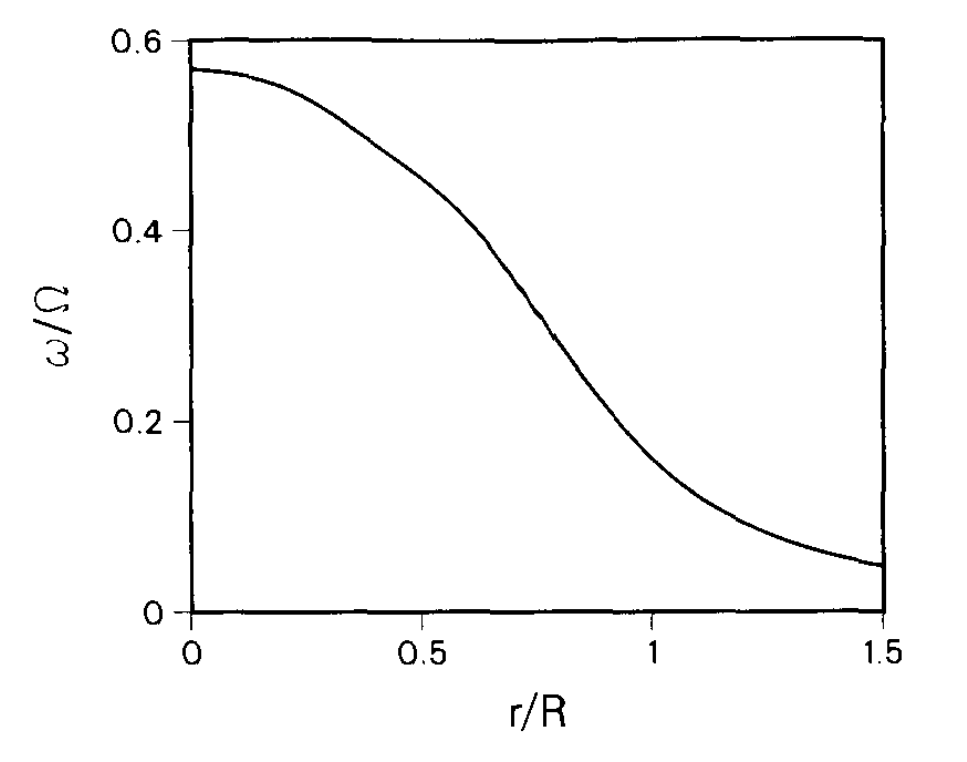
\includegraphics[width=0.45\linewidth]{./images/ns-omega.png}
\end{figure}

\end{frame}

%----------------------------------------------------------------------------------------
%	SLIDE 8.
%----------------------------------------------------------------------------------------
\begin{frame}
\frametitle{Solutions for relativistic stars}
\framesubtitle{Motivation}

\begin{exampleblock}{Problems with previous solutions}
	\begin{itemize}
		\item The equation \eqref{eq:8} is only valid for static or slowly rotating objects.
		\item Rotation introduces $\theta$ dependence of $\omega$.
		\item Different attributes of the system (change in angular momentum, change in centrifugal forces, changes in the shape of the star etc.) are all intertwined.
	\end{itemize}
\end{exampleblock}

\begin{alertblock}{How to approach these problems?}
	All the phenomenons and quantities mentioned above are connected by $I$, the moment of inertia of the star, hence we're interested in the description of this quantity.
\end{alertblock}

\end{frame}

%----------------------------------------------------------------------------------------
%	SLIDE 9.
%----------------------------------------------------------------------------------------
\begin{frame}
\frametitle{Solutions for relativistic stars}
\framesubtitle{Derivation}

\begin{itemize}
	\item The z-component (the axis of rotation) of the angular momentum can be computed as
	\begin{block}{}
		\begin{equation}
			J
			=
			I \Omega
			=
			\int \mathrm{d}r\,\mathrm{d}\theta\,\mathrm{d}\phi\,
			\sqrt{- \det g_{\alpha \beta}} T^{t}_{\phi}
		\end{equation}
	\end{block}
	\item Our goal is to determine the determinant $g$ of the metric tensor $g_{\alpha \beta}$ and the mass-energy tensor $T$ to be able to calculate the $J$ angular momentum and the $I$ moment of inertia. After some algebra we get the final form for $J$ and subsequently for $I$:
	\begin{block}{}
		\begin{equation}
			J
			=
			I \Omega
			=
			- \int \mathrm{d}r\,\mathrm{d}\theta\,\mathrm{d}\phi\,
			\frac{
				\left( p + \epsilon \right) \left( \Omega - \omega \right) r^{4} \sin^{3} \left( \theta \right) e^{\nu + \lambda + 2 \mu}
			}{
				e^{2 \left( \nu - \mu \right)}
				-
				r^{2} \sin^{2} \left( \theta \right) \left( \Omega - \omega \right)^{2}
			}
		\end{equation}
	\end{block}
\end{itemize}

\end{frame}

%----------------------------------------------------------------------------------------
%	SLIDE 10.
%----------------------------------------------------------------------------------------
\begin{frame}
\frametitle{Realistic nuclear matter equation of state (EoS)}

\begin{itemize}
	\item The goal of constructing an EoS is to describe the thermodynamical properties (mainly the energy density $\epsilon$ and the pressure $p$) of the nuclear matter that the NS consists of.
	\item The crust and core of the NS usually described using different models.
	\item There is a real abundance of models trying to describe NS in any way. In the modern NS literature, models based on relativistic mean-field theory became the most widely used ones.
	\item In Glendenning's Compact stars there are 17 different EoS mentioned and compared with each other (pp. 296--297, Table 6.3 and 6.4).
\end{itemize}
\begin{alertblock}{Main question}
	\centering	
	What are the real constraints on the EoS?
\end{alertblock}

\end{frame}

%\placelogofalse
%\placelogotrue

\end{document} 